 \section{Supplementary figures}
 \begin{figure*}[ht]
 \centering
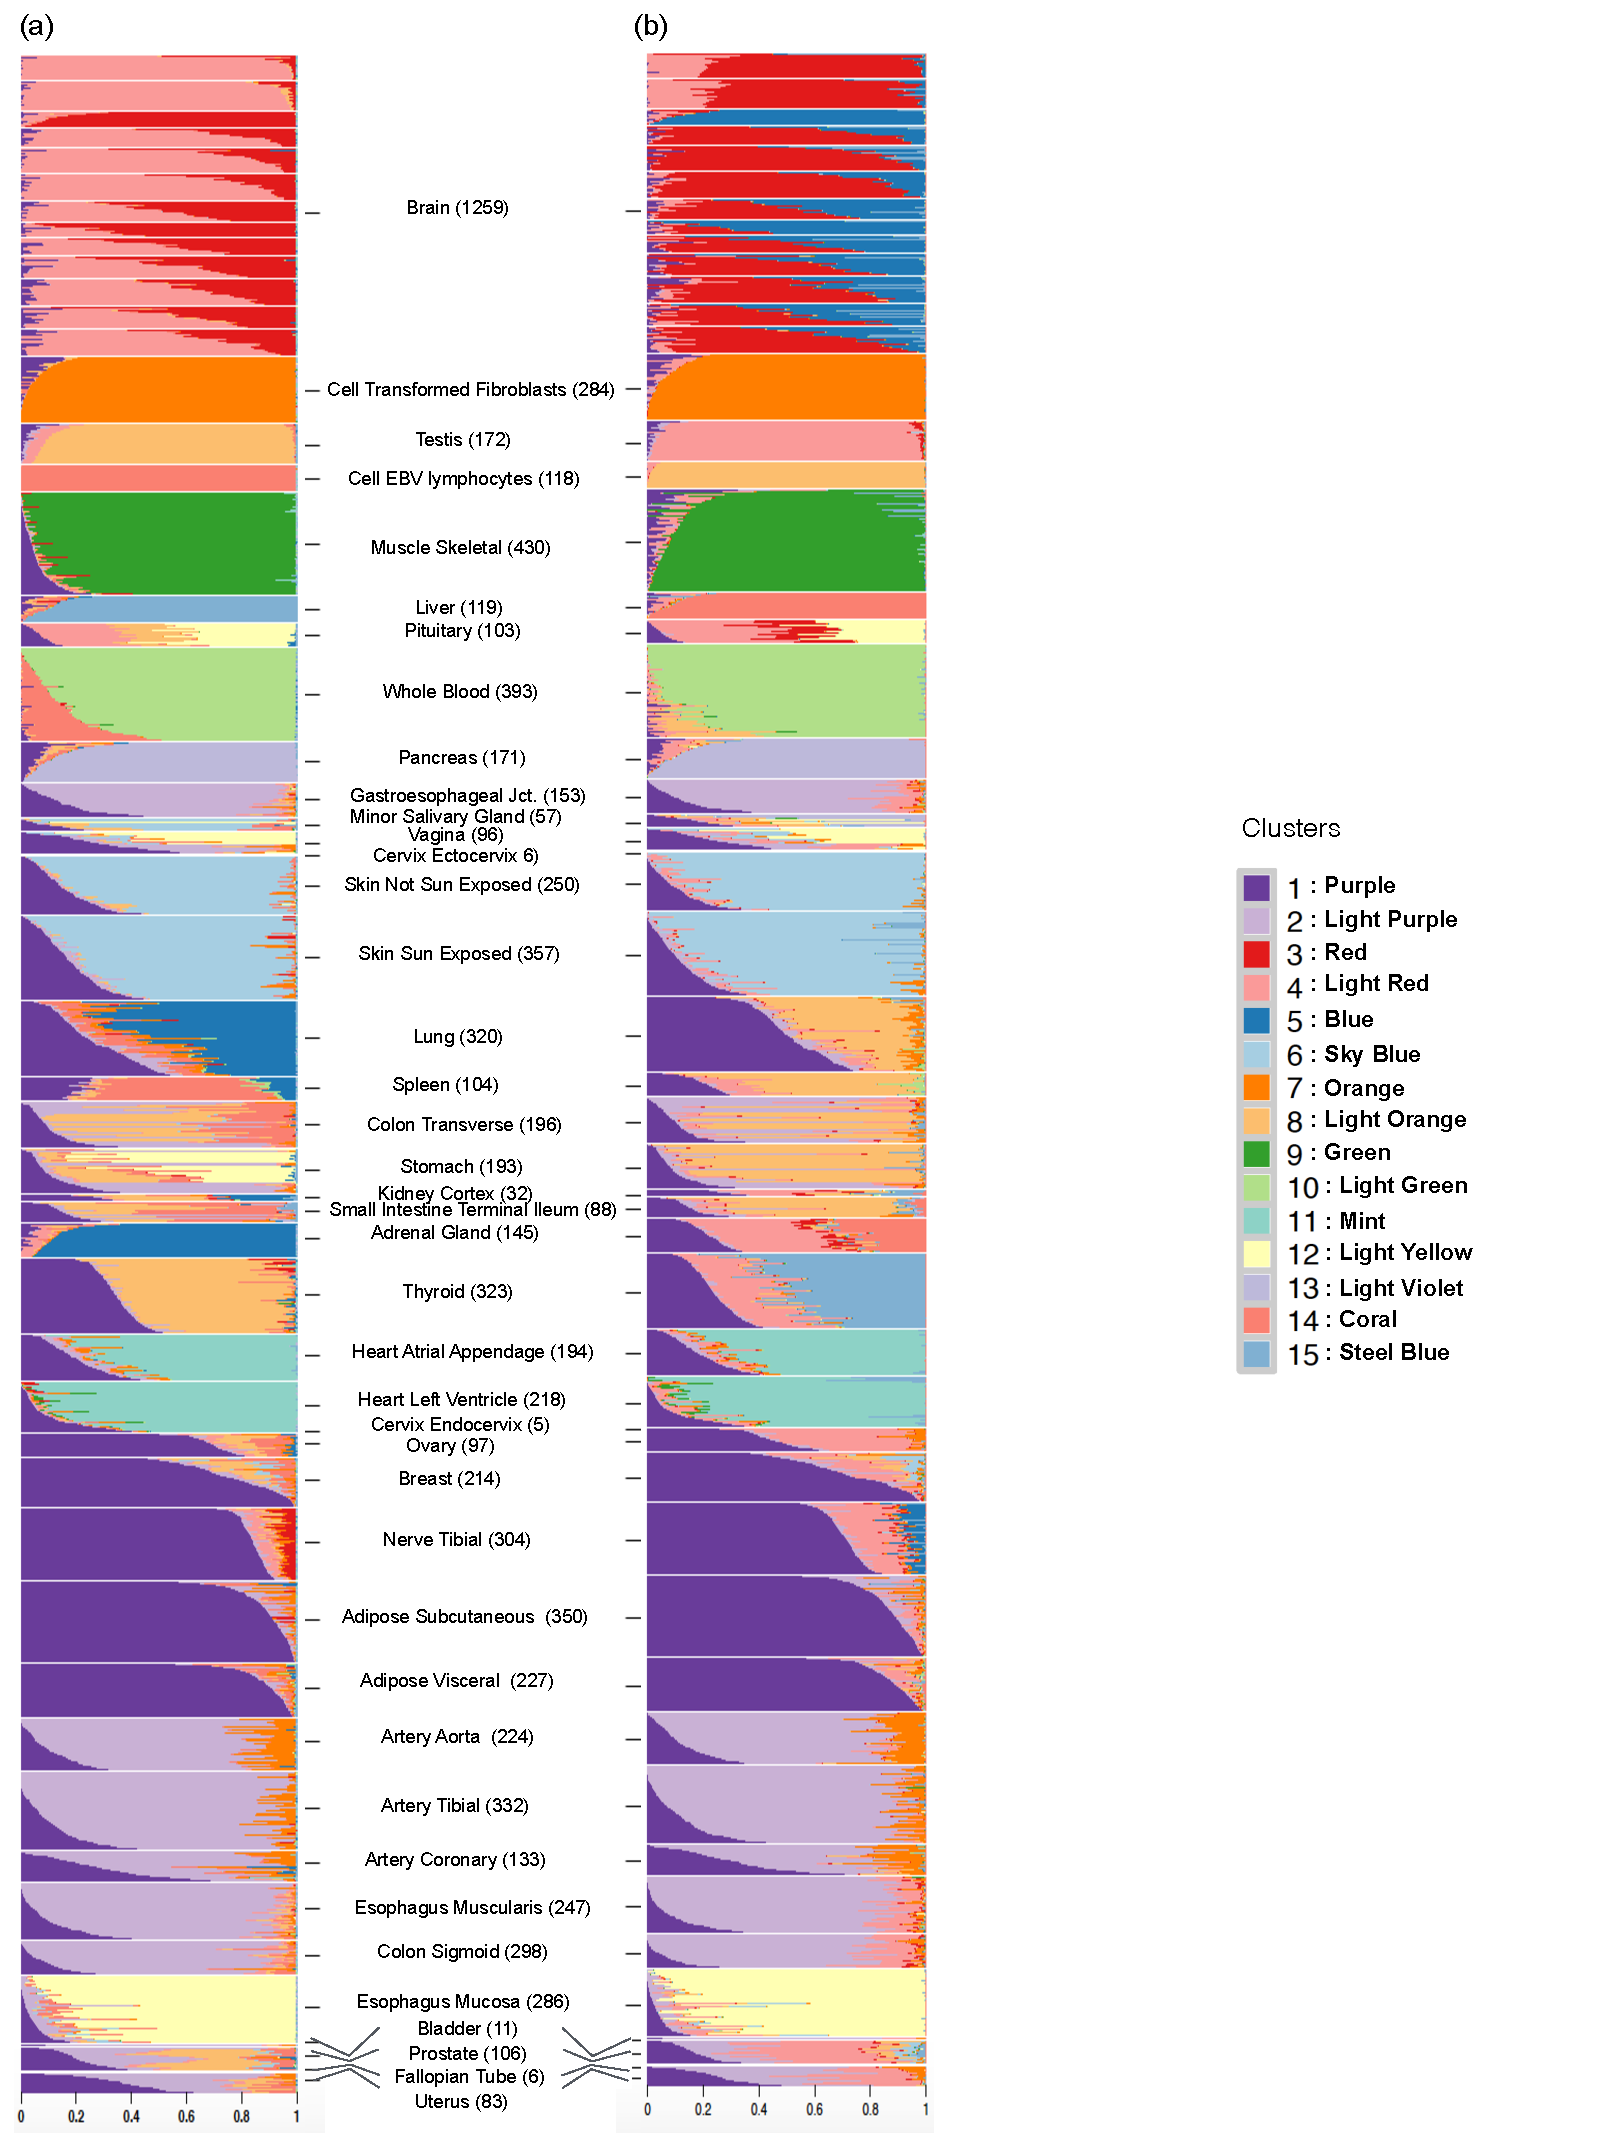
\includegraphics[height=7.5in, width=6.5in]{../plots/gtex-figures/gtex2_02_29_16.pdf}
    \caption{Structure plot of all tissue samples in 2 runs of the GTEx V6 data for  K=15 for the thinning parameters (a) $p_{thin}=0.01$ and (b) $p_{thin}=0.0001$. The patterns in two plots closely correspond to the plot in \textbf{Fig} ~\ref{fig:fig1} (a), though are a bit more noisy than compared to the unthinned version. }
 \label{fig:figS1}
    \end{figure*}

 \begin{figure*}[ht]
    \centering    
     \begin{subfigure}[t]{0.5\textwidth}
        \centering
        \includegraphics[height=2.5in]{../plots/rsz_1hierarchy_F_thin_0_01.png}
        \caption{hierarchy thin 0.01}
    \end{subfigure}%
    ~
    \begin{subfigure}[t]{0.5\textwidth}
        \centering
        \includegraphics[height=2.5in]{../plots/rsz_1admixture_F_thin_0_01.png}
        \caption{GoM thin 0.01}
    \end{subfigure}\\
    
     \begin{subfigure}[t]{0.5\textwidth}
        \centering
        \includegraphics[height=2.5in]{../plots/rsz_1hierarchy_F_thin_0_0001.png}
        \caption{hierarchy 0.0001}
    \end{subfigure}%
    ~
    \begin{subfigure}[t]{0.5\textwidth}
        \centering
        \includegraphics[height=2.5in]{../plots/rsz_1admixture_F_thin_0_0001.png}
        \caption{GoM thin 0.0001}
    \end{subfigure}\\

 \caption{A comparison of ``accuracy" of hierarchical vs model-based clustering on thinned GTEx data, with thinning parameter $p_{thin}=0.01$ and $p_{thin}=0.0001$.  For each pair of tissues from the GTEx data we assessed whether or not each clustering method (with $K=2$ clusters) separated the samples according to their actual tissue of origin, with successful separation indicated by a filled square. Thinning deteriorates accuracy compared with the unthinned data (Figure \ref{fig:fig2}), but even then the model-based method remains more successful than the hierarchical clustering in separating the samples by tissue or origin.}
 \label{fig:figS2}
\end{figure*}
\clearpage
